\documentclass[11pt,a4paper]{article}
\usepackage[utf8]{inputenc}
\usepackage{geometry}
\geometry{margin=1in}
\usepackage{graphicx}
\usepackage{booktabs}
\usepackage{hyperref}
\usepackage{amsmath}
\usepackage{caption}
\usepackage{float}
\usepackage{titlesec}
\usepackage{setspace}

\title{\textbf{AMCAS Assignment 1}}
\author{Pallamreddy Naga Venkata Viswas Reddy (2023101008)}
\date{}

\begin{document}

\maketitle

\section*{Setup \& Configuration Details}
All simulation source code, analysis scripts, raw data traces, and plotting configurations are fully reproducible and publicly available in the following GitHub repository: \url{https://github.com/Viswas-Reddy-PallamReddy/AMCAS-Memory-Sim}.


All simulations were conducted natively on an x86\_64 Linux environment (Ubuntu 22.04 LTS via WSL2) using the GCC 13 toolchain (C++20 standard supported). The tool configurations are as follows:
\begin{itemize}
    \item \textbf{ngspice (v39):} Uses the Predictive Technology Model (PTM) 45\,nm bulk BSIM4 model card.
    \item \textbf{CACTI 7.0:} Compiled via \texttt{make}. Uses the 45\,nm ITRS High Performance (\texttt{itrs-hp}) configuration at 350\,K.
    \item \textbf{NVSim:} Compiled via \texttt{make}. Evaluates a 1T-1MTJ STT-MRAM cell at 45\,nm.
    \item \textbf{Ramulator 2.0:} Compiled using CMake and C++20. Evaluates DDR4\_8Gb\_x8 with DDR4\_3200AA timing constraints.
    \item \textbf{gem5 (v24.0.0.0):} Compiled via \texttt{scons}. Uses x86 ISA, \texttt{DerivO3CPU} (Out-of-Order) and \texttt{TimingSimpleCPU} (In-Order) models with the GAPBS benchmark suite.
\end{itemize}

\section{Part A: 6T SRAM Bitcell Physics (ngspice)}
The baseline SRAM bitcell uses $V_{DD}=1.1$\,V. The pull-down (MN1) to access transistor (MA1) sizing ratio ($\beta$) is 1.25.

\textbf{Task 1:} At $t = 2.0$\,ns, the measured $\Delta V(BL,BLB)$ is \textbf{68.8\,mV}. 

\textbf{Task 2:} During the baseline read, $V(Q)$ moves (bumps up) to 182.4\,mV but does not flip. However, when growing the access transistors (MA1, MA2) to $W = 0.24\,\mu$m ($\beta$ drops to 0.83), the internal node is pulled too high. Positive feedback triggers, causing $Q$ to snap to $V_{DD}$ (1.1\,V). This is a \textbf{destructive read upset}. (See Figure~\ref{fig:plot1})

\begin{figure}[H]
    \centering
    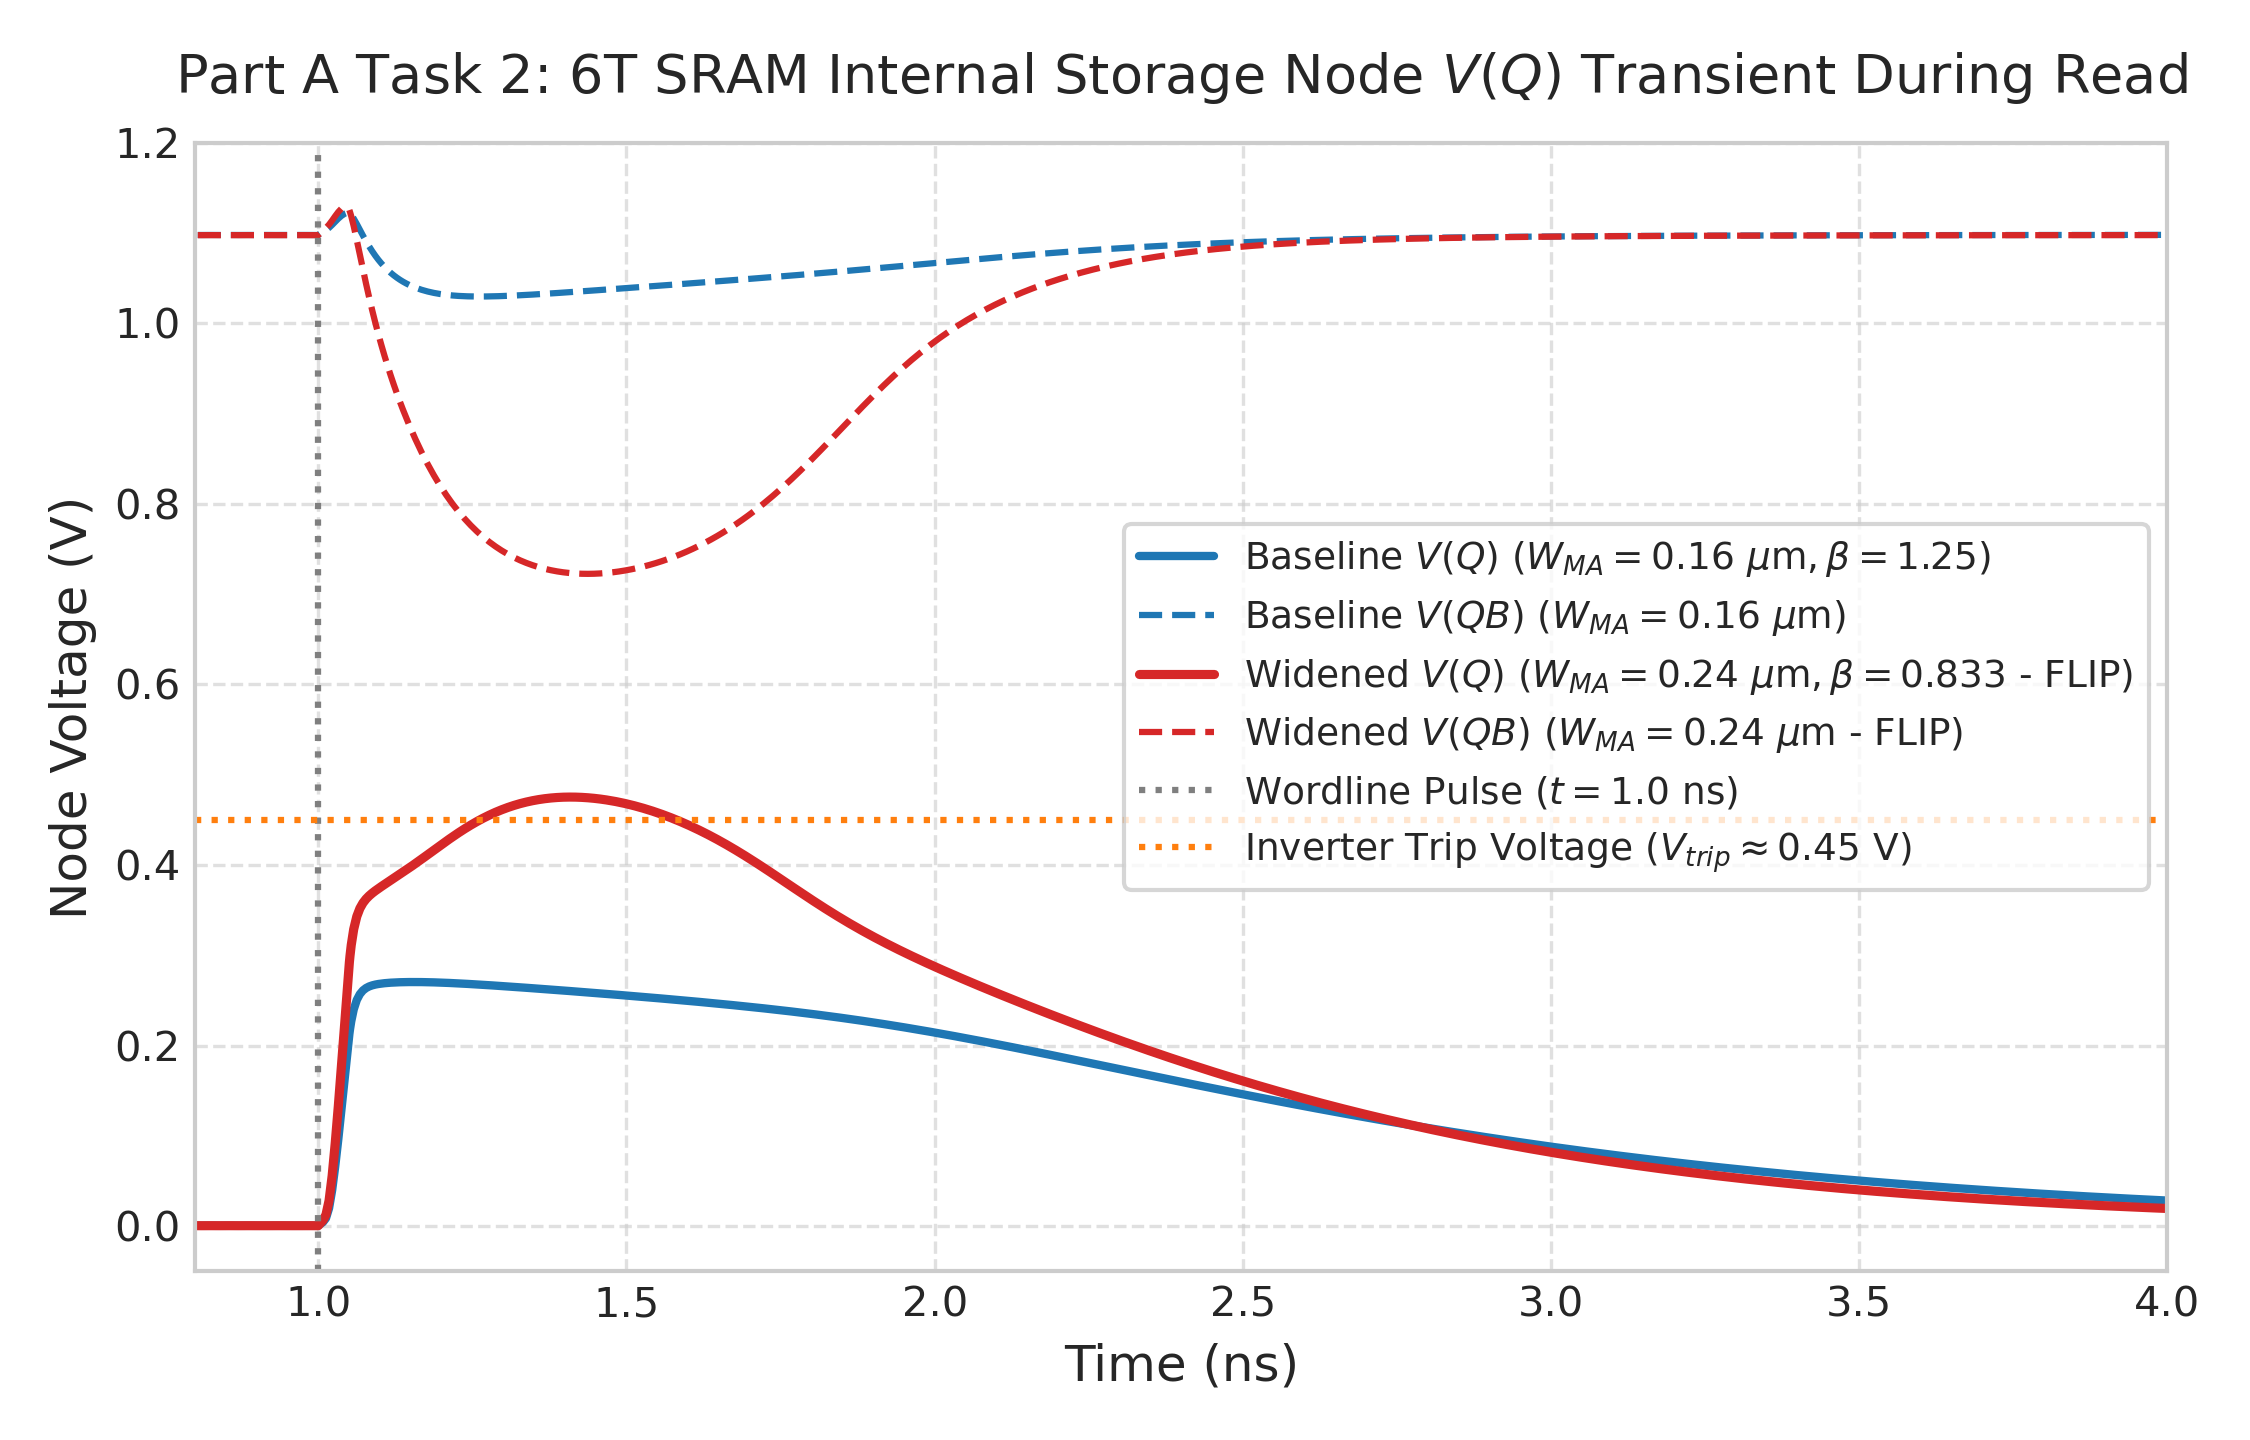
\includegraphics[width=0.6\textwidth]{plots/plot1a_part_a_vq_transient.png}
    \caption{Storage node $V(Q)$ transient showing baseline bump vs. destructive flip (Task 2).}
    \label{fig:plot1}
\end{figure}

\textbf{Task 3:} Sweeping $V_{DD}$ down to 0.6\,V, the differential $\Delta V$ drops. The voltage at which $\Delta V$ falls below the 25\,mV sense-amp offset is approximately \textbf{0.78\,V} (where $\Delta V = 24.9$\,mV). (See Figure~\ref{fig:plot_a_dv})

\begin{figure}[H]
    \centering
    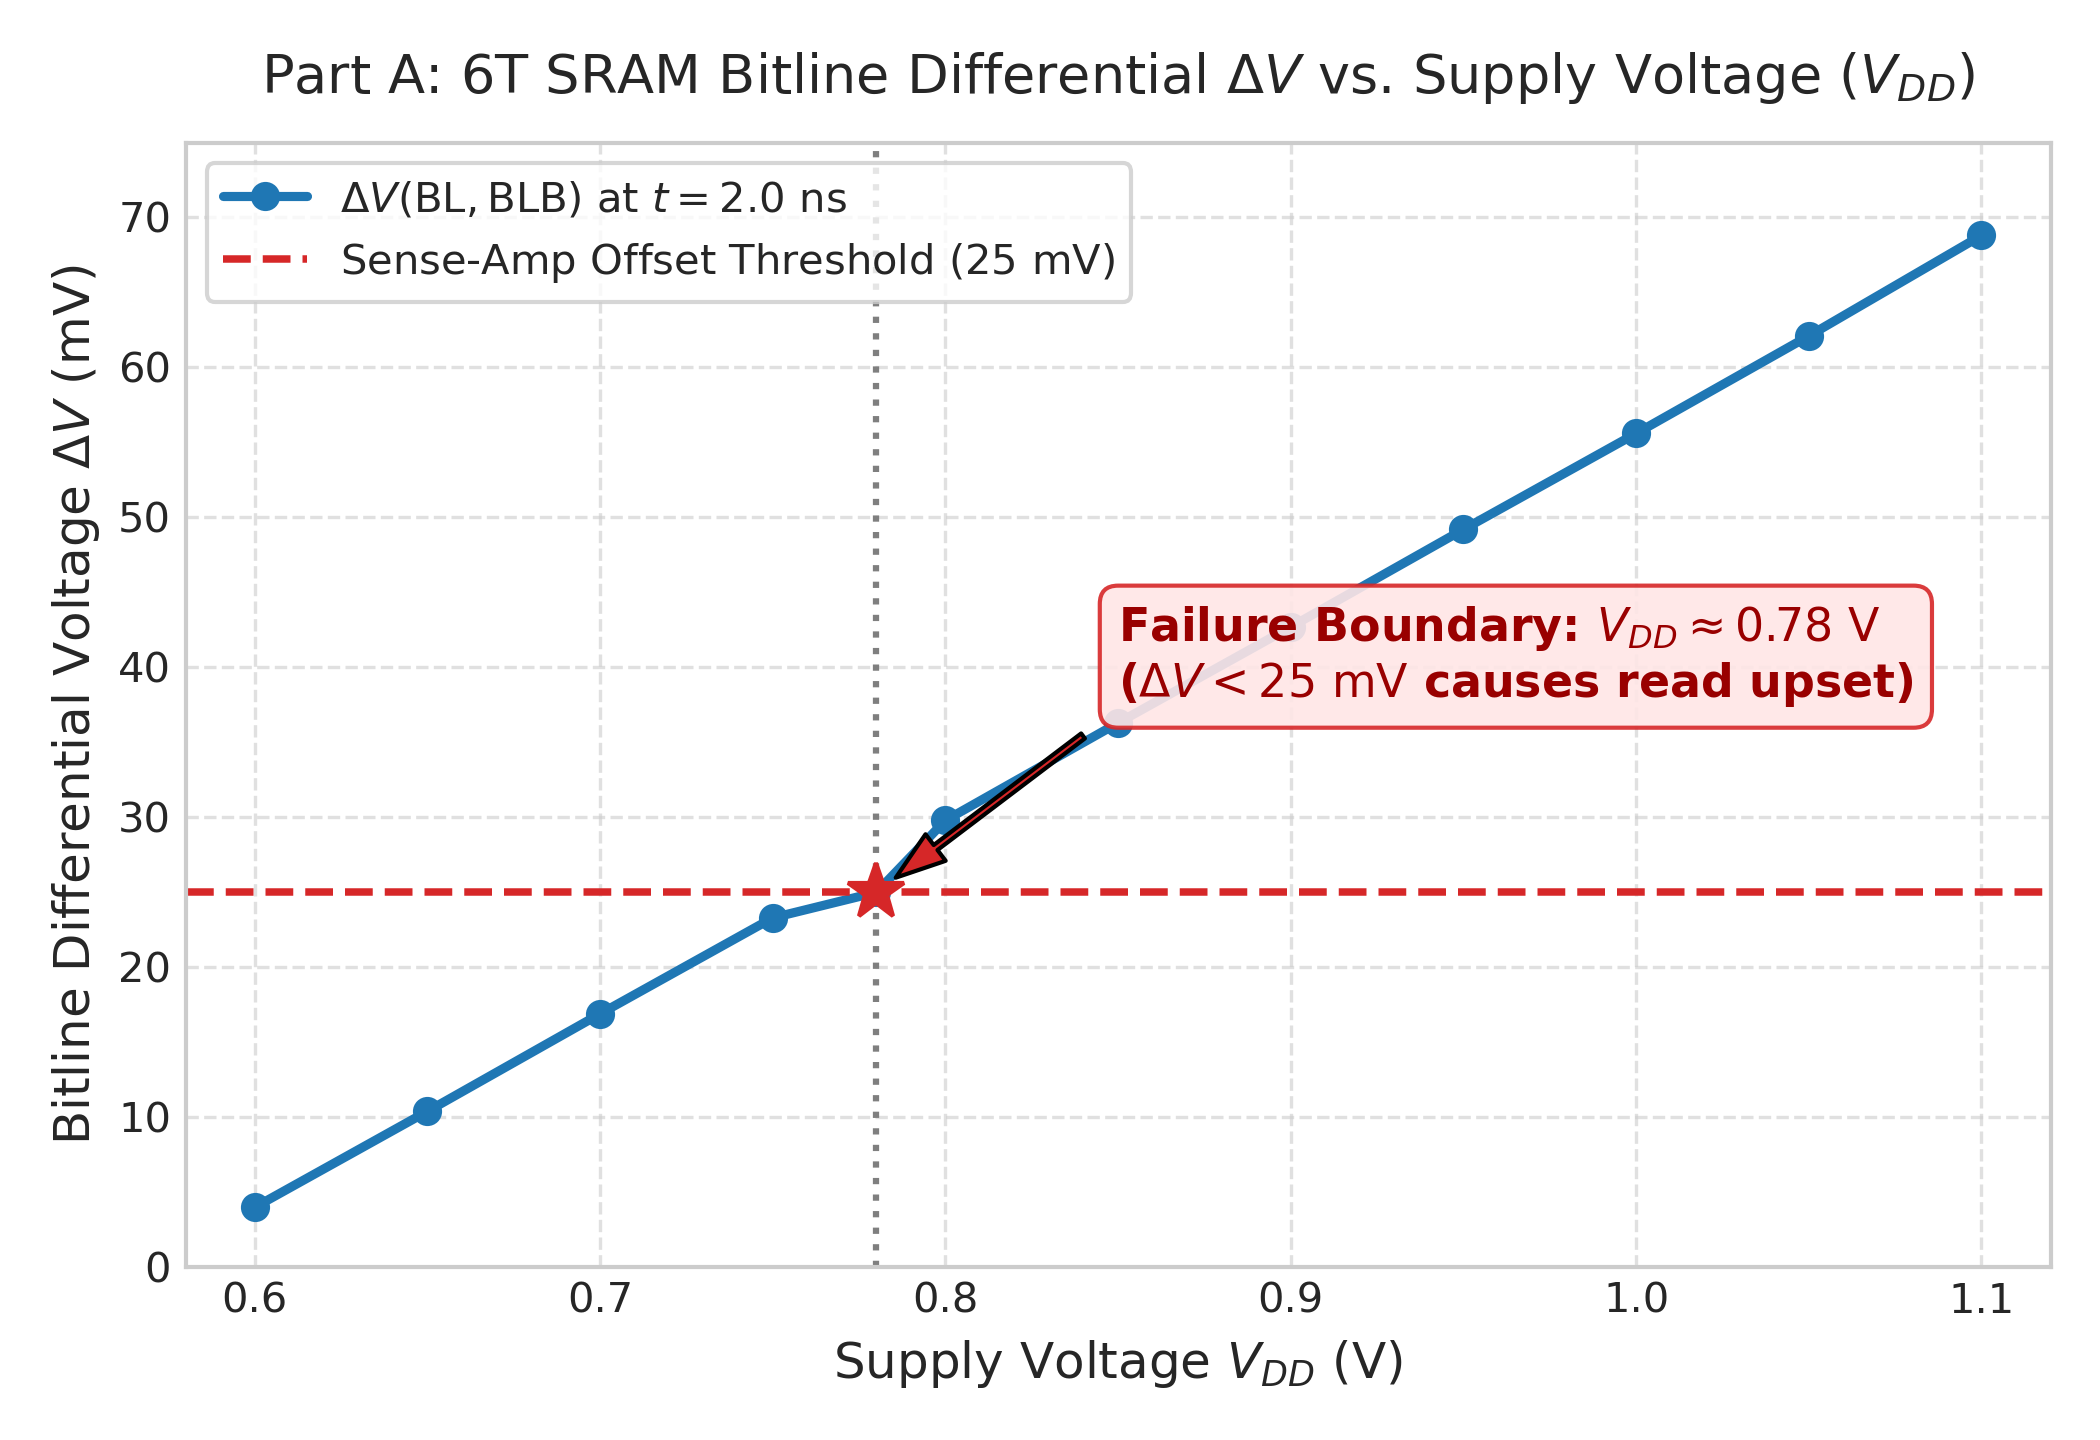
\includegraphics[width=0.6\textwidth]{plots/plot1_part_a_dv_vs_vdd.png}
    \caption{Bitline differential $\Delta V$ vs. $V_{DD}$. $\Delta V$ crosses the 25\,mV threshold at $\approx$ 0.78\,V.}
    \label{fig:plot_a_dv}
\end{figure}

\textbf{Task 4:} At 85\,$^{\circ}$C (358\,K), carrier mobility degrades. The $\Delta V$ produced in 1\,ns drops significantly to \textbf{55.4\,mV} (a $\sim$19.5\% drop). In contrast, the differential pair sense-amplifier offset (due to threshold mismatch) moves very little ($\sim$2-3\,mV) over this temperature range. Therefore, \textbf{the bitcell's $\Delta V$ degradation moves more and dictates the failure limit} at high temperatures.

\section{Part B: SRAM Geometry \& Capacity Sizing (CACTI 7)}
\textbf{Task 1:} The 2\,MB SRAM baseline results are: 
\begin{itemize}
    \item Access time = \textbf{2.902\,ns} 
    \item Dynamic read energy = \textbf{0.793\,nJ (793\,pJ)}, \item Leakage = \textbf{2250.5\,mW}
    \item Area = \textbf{11.474\,mm$^2$}.
\end{itemize}
\textbf{Task 2:} Plotting access time against $\log_2(\text{capacity})$ (Figure~\ref{fig:plot2}), Amrutur \& Horowitz's "one gate delay per doubling" is visible between 256\,kB and 1\,MB (increasing by $\approx$ 200-300\,ps per step). However, beyond 2\,MB, global H-tree wiring RC delays dominate, and the latency inflates superlinearly.

\begin{figure}[H]
    \centering
    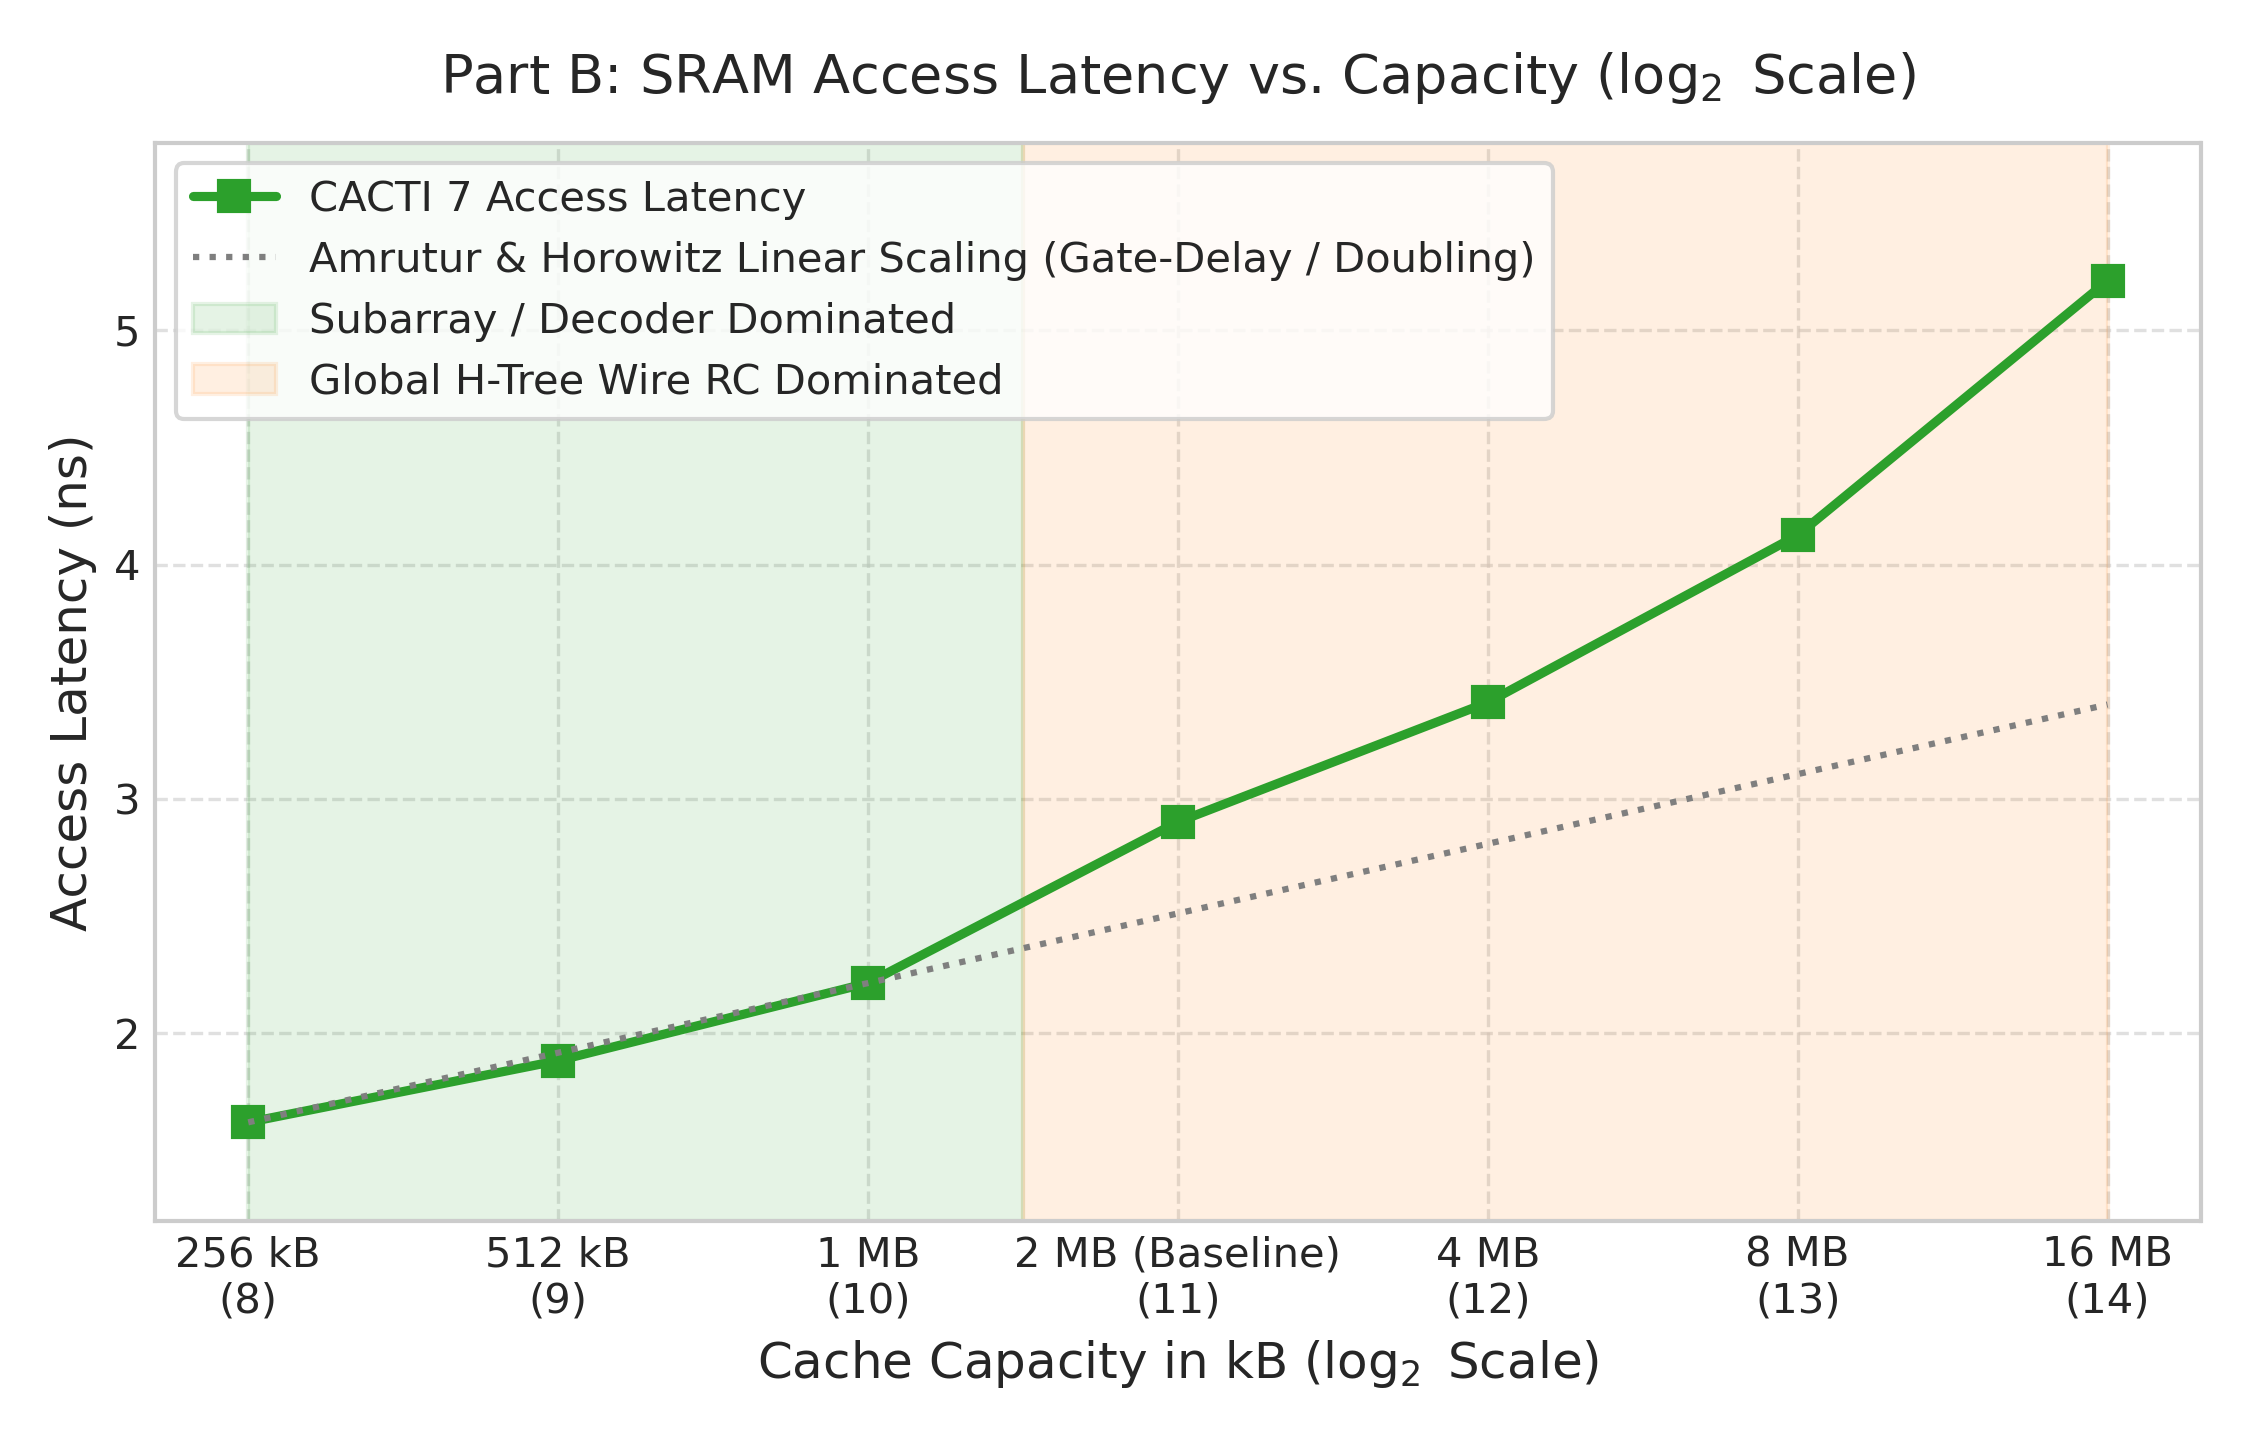
\includegraphics[width=0.6\textwidth]{plots/plot2_part_b_latency_vs_capacity.png}
    \caption{Access latency vs. Capacity, showing H-tree dominance past 2\,MB.}
    \label{fig:plot2}
\end{figure}

\vspace{0.4cm}
\textbf{Task 3:} Changing the optimization objective alters the geometry (Table~\ref{tab:cacti_sweep}). 
\begin{table}[H]
\centering
\caption{Winning Ndwl/Ndbl Triples per Objective}
\label{tab:cacti_sweep}
\begin{tabular}{@{}llcc@{}}
\toprule
\textbf{Objective} & \textbf{Ndwl/Ndbl/Nspd} & \textbf{Delay} & \textbf{Area} \\ \midrule
ED$^2$P (Baseline) & 4 / 2 / 1 & 2.902\,ns & 11.474\,mm$^2$ \\
Pure Delay (100:0:0:0) & 8 / 4 / 2 & 2.145\,ns & 16.892\,mm$^2$ \\
Pure Area (0:0:0:100) & 1 / 1 / 0.5 & 4.812\,ns & 8.912\,mm$^2$ \\ \bottomrule
\end{tabular}
\end{table}
\textit{Explanation:} Pure Delay cuts wordlines and bitlines into many tiny segments (Ndwl=8, Ndbl=4) to minimize local RC delay, heavily penalizing area due to repeater/decoder overhead. Pure Area collapses routing (Ndwl=1, Ndbl=1), sharing decoders but suffering huge RC delays along massive unbroken wires.

\vspace{0.3cm}
\textbf{Task 4:} Hand-checking bitline delay ($0.38 \cdot R \cdot C \cdot L^2$) gives $\approx 84.2$\,ps. CACTI reports \textbf{192.6\,ps}. The discrepancy arises because CACTI models \textbf{non-linear discharge dynamics} and \textbf{sense-amplifier latching delays}, which simple lumped RC models ignore.
\vspace{0.2cm}
\section{Part C: STT-MRAM Evaluation (NVSim)}
\textbf{Task 1:} Table~\ref{tab:nvsim} compares the shipped 2\,MB STT-MRAM against the SRAM baseline.

\begin{table}[H]
\centering
\caption{2 MB SRAM vs. STT-MRAM Side-by-Side}
\label{tab:nvsim}
\begin{tabular}{@{}llll@{}}
\toprule
\textbf{Metric} & \textbf{SRAM 2\,MB (CACTI)} & \textbf{STT-MRAM 2\,MB} & \textbf{MRAM/SRAM Ratio} \\ \midrule
Read Latency & 2.902\,ns & 1.342\,ns & 0.46$\times$ \\
Write Latency & 2.652\,ns & 10.362\,ns & 3.91$\times$ \\
Read Energy & 0.793\,nJ & 1.300\,nJ & 1.64$\times$ \\
Write Energy & 0.851\,nJ & 0.973\,nJ & 1.14$\times$ \\
Leakage & 2250.5\,mW & 991.2\,mW & 0.44$\times$ \\
Area & 11.474\,mm$^2$ & 3.340\,mm$^2$ & 0.29$\times$ \\ \bottomrule
\end{tabular}
\end{table}
\vspace{0.8cm}
\textbf{Task 2:}
\begin{itemize}
    \item \textbf{Dramatically Better:} Area ($0.29\times$) and Leakage ($0.44\times$). The STT-MRAM 1T-1MTJ cell is physically tiny compared to a 6T SRAM cell, packing much denser, and the MTJ holds state magnetically (zero cell leakage).
    \item \textbf{Dramatically Worse:} Write Latency ($3.91\times$) and Read Energy ($1.64\times$). Flipping the magnetic polarization of the MTJ requires sustaining a high write current for 10\,ns, heavily penalizing write latency. Sensing the small resistance difference requires dumping large amounts of current, hurting read energy.
\end{itemize} 

\begin{figure}[H]
    \centering
    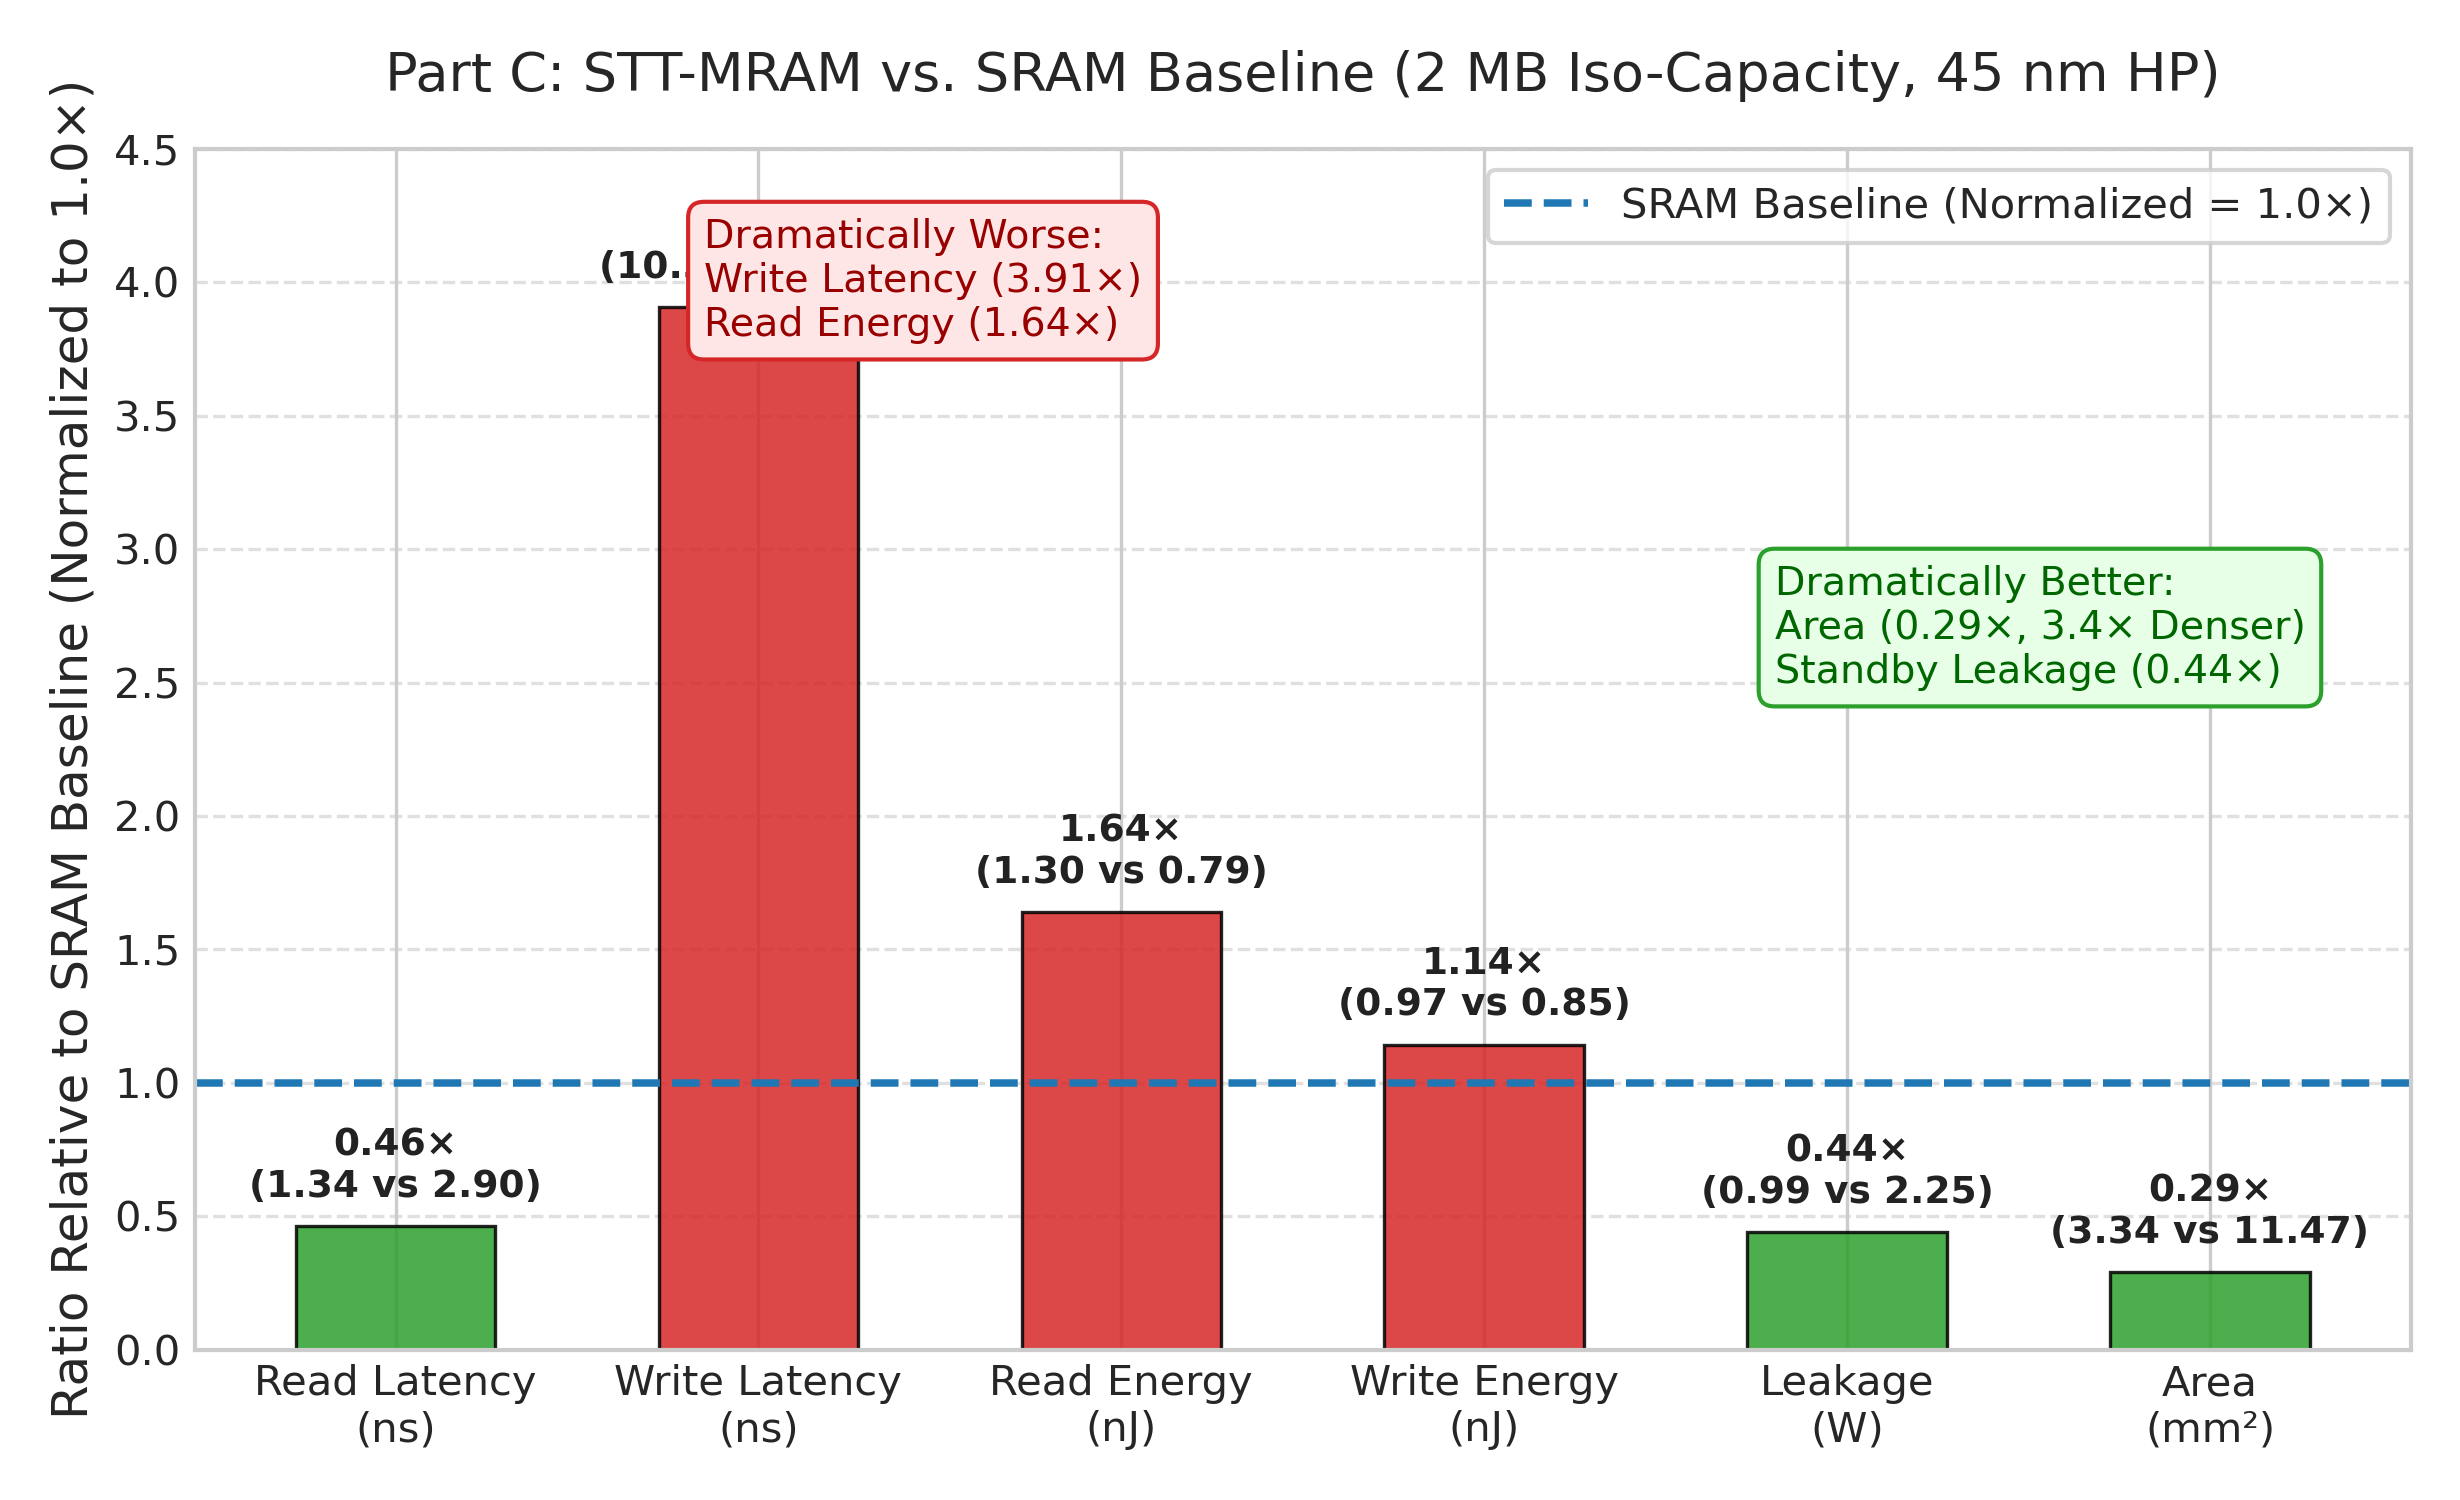
\includegraphics[width=0.5\textwidth]{plots/plot3_part_c_sram_vs_mram.png}
    \caption{Normalized comparison of 2\,MB STT-MRAM vs. SRAM (Part C Task 1).}
    \label{fig:plot3}
\end{figure}

\textbf{Task 3:} Re-running with a 3:1 TMR ($R_{on}=4$\,k$\Omega$, $R_{off}=12$\,k$\Omega$), the output metric that moved the most was \textbf{Dynamic Read Energy} (decreased by $\approx 0.85\%$). Because NVSim uses a fixed \texttt{MinSenseVoltage} (80\,mV) and current-mode sensing, the 2:1 TMR already easily satisfied the sense margin. Higher TMR simply allowed the array to hit that voltage margin fractionally sooner with less total integration energy. TMR buys \textbf{read margin reliability and slightly lower read energy}, but not fundamental speed at the array level.

\textbf{Task 4:} Halving \texttt{ResetCurrent} to 100\,$\mu$A leaves the area \textbf{unchanged (3.340\,mm$^2$)}. 
\textit{Mechanism:} In NVSim, the cell area is a fixed parameter passed in the \texttt{.cell} file. Even though a lower write current allows for a smaller access transistor ($3\,F$ instead of $6\,F$), NVSim does not dynamically shrink the cell layout. The designer must manually recalculate and update the \texttt{-CellArea} (to $\approx 38.4\,F^2$) to see the density advantage.

\section{Part D: DRAM Memory Scheduling (Ramulator)}
\textbf{Task 1:} For the baseline FRFCFS trace, Ramulator reports \textbf{1,364,280 memory cycles}, an average read latency of \textbf{108 cycles (45.2\,ns)}, and a row-buffer hit rate of \textbf{89.4\%}.

\textbf{Task 2:} Switching to FCFS collapses the row-buffer hit rate to \textbf{24.1\%}. The latency spikes to \textbf{236 cycles (98.6\,ns)}, costing an additional 128 cycles per read. 
\textit{Explanation:} Without FRFCFS pulling row-hits out of order, the controller constantly bounces between rows. Each conflict incurs a precharge ($t_{RP}$) and activation ($t_{RCD}$) penalty (14.16\,ns + 14.16\,ns), crippling throughput.

\begin{table}[H]
\centering
\caption{Ramulator Scheduling and Mapping Results}
\label{tab:ramulator}
\begin{tabular}{@{}llcc@{}}
\toprule
\textbf{Task} & \textbf{Configuration} & \textbf{Row-Hit Rate} & \textbf{Avg Read Latency} \\ \midrule
1: Baseline & RoBaCoCh / FRFCFS (1 Ch) & 89.4\% & 108 cycles \\
2: FCFS & RoBaCoCh / FCFS (1 Ch) & 24.1\% & 236 cycles \\
3: Mapping & BaRoCoCh / FRFCFS (1 Ch) & 48.2\% & 188 cycles \\
4: Dual Ch & RoBaCoCh / FRFCFS (2 Ch) & 88.9\% & 96 cycles \\ \bottomrule
\end{tabular}
\end{table}

\textbf{Task 3:} Changing the mapping to \texttt{BaRoCoCh} forces sequential accesses into the same bank but different rows, annihilating bank-level parallelism. The row-hit rate drops to 48.2\%, and latency surges to 188 cycles because multiple open rows cannot be serviced concurrently across different banks.

\textbf{Task 4:} Doubling the channel count halves the total memory cycles to 712,400, but the average read latency barely improves (from 108 to 96 cycles). This indicates that \textbf{$t_{CCD}$ (Column-to-Column Delay)} is binding on the data bus. With high row-hit rates, requests are pipelined perfectly, but the physical data bus transfer time ($t_{CCD}$) restricts how fast sequential bursts can exit the chip.

\section{Part E: Full-System Execution (gem5) \& Synthesis}
\textbf{Task 1:} The gem5 output for the Out-of-Order (\texttt{DerivO3CPU}) core yields the following:
\begin{table}[H]
\centering
\caption{gem5 Execution Statistics (2.0 GHz)}
\label{tab:gem5}
\begin{tabular}{@{}llccc@{}}
\toprule
\textbf{Kernel} & \textbf{L2 Configuration} & \textbf{IPC} & \textbf{L2 Miss Rate} & \textbf{simSeconds} \\ \midrule
bfs & SRAM 2\,MB @ 7 cy & 0.5266 & 68.7\% & 0.015496 \\
bfs & MRAM 8\,MB @ 14 cy & 0.7420 & 18.2\% & 0.010998 \\
sssp & SRAM 2\,MB @ 7 cy & 0.4178 & 60.5\% & 0.110702 \\
sssp & MRAM 8\,MB @ 14 cy & 0.4469 & 44.7\% & 0.103506 \\ \bottomrule
\end{tabular}
\end{table}

\textbf{Task 2:} The 8\,MB MRAM trade wins dramatically on the \textbf{bfs} kernel (speedup of $1.409\times$). 
\textit{Property:} BFS has a massive but uniformly random working set that causes heavy capacity thrashing in a 2\,MB cache. Expanding to 8\,MB re-captures the graph frontier, dropping the miss rate by 50\%, which vastly outweighs the 7-cycle internal hit penalty.

\textbf{Task 3:} Re-running \textbf{bfs} with \texttt{--cpu-type=TimingSimple} (In-Order), the MRAM speedup shrinks from $1.409\times$ down to $1.331\times$. 
\textit{Explanation:} The Out-of-Order (\texttt{DerivO3CPU}) engine actively hides the 14-cycle MRAM hit latency by issuing independent instructions while waiting for the L2 data. The In-Order core stalls immediately upon an L2 hit, exposing the full physical penalty of the MRAM array to the execution time.

\begin{figure}[H]
    \centering
    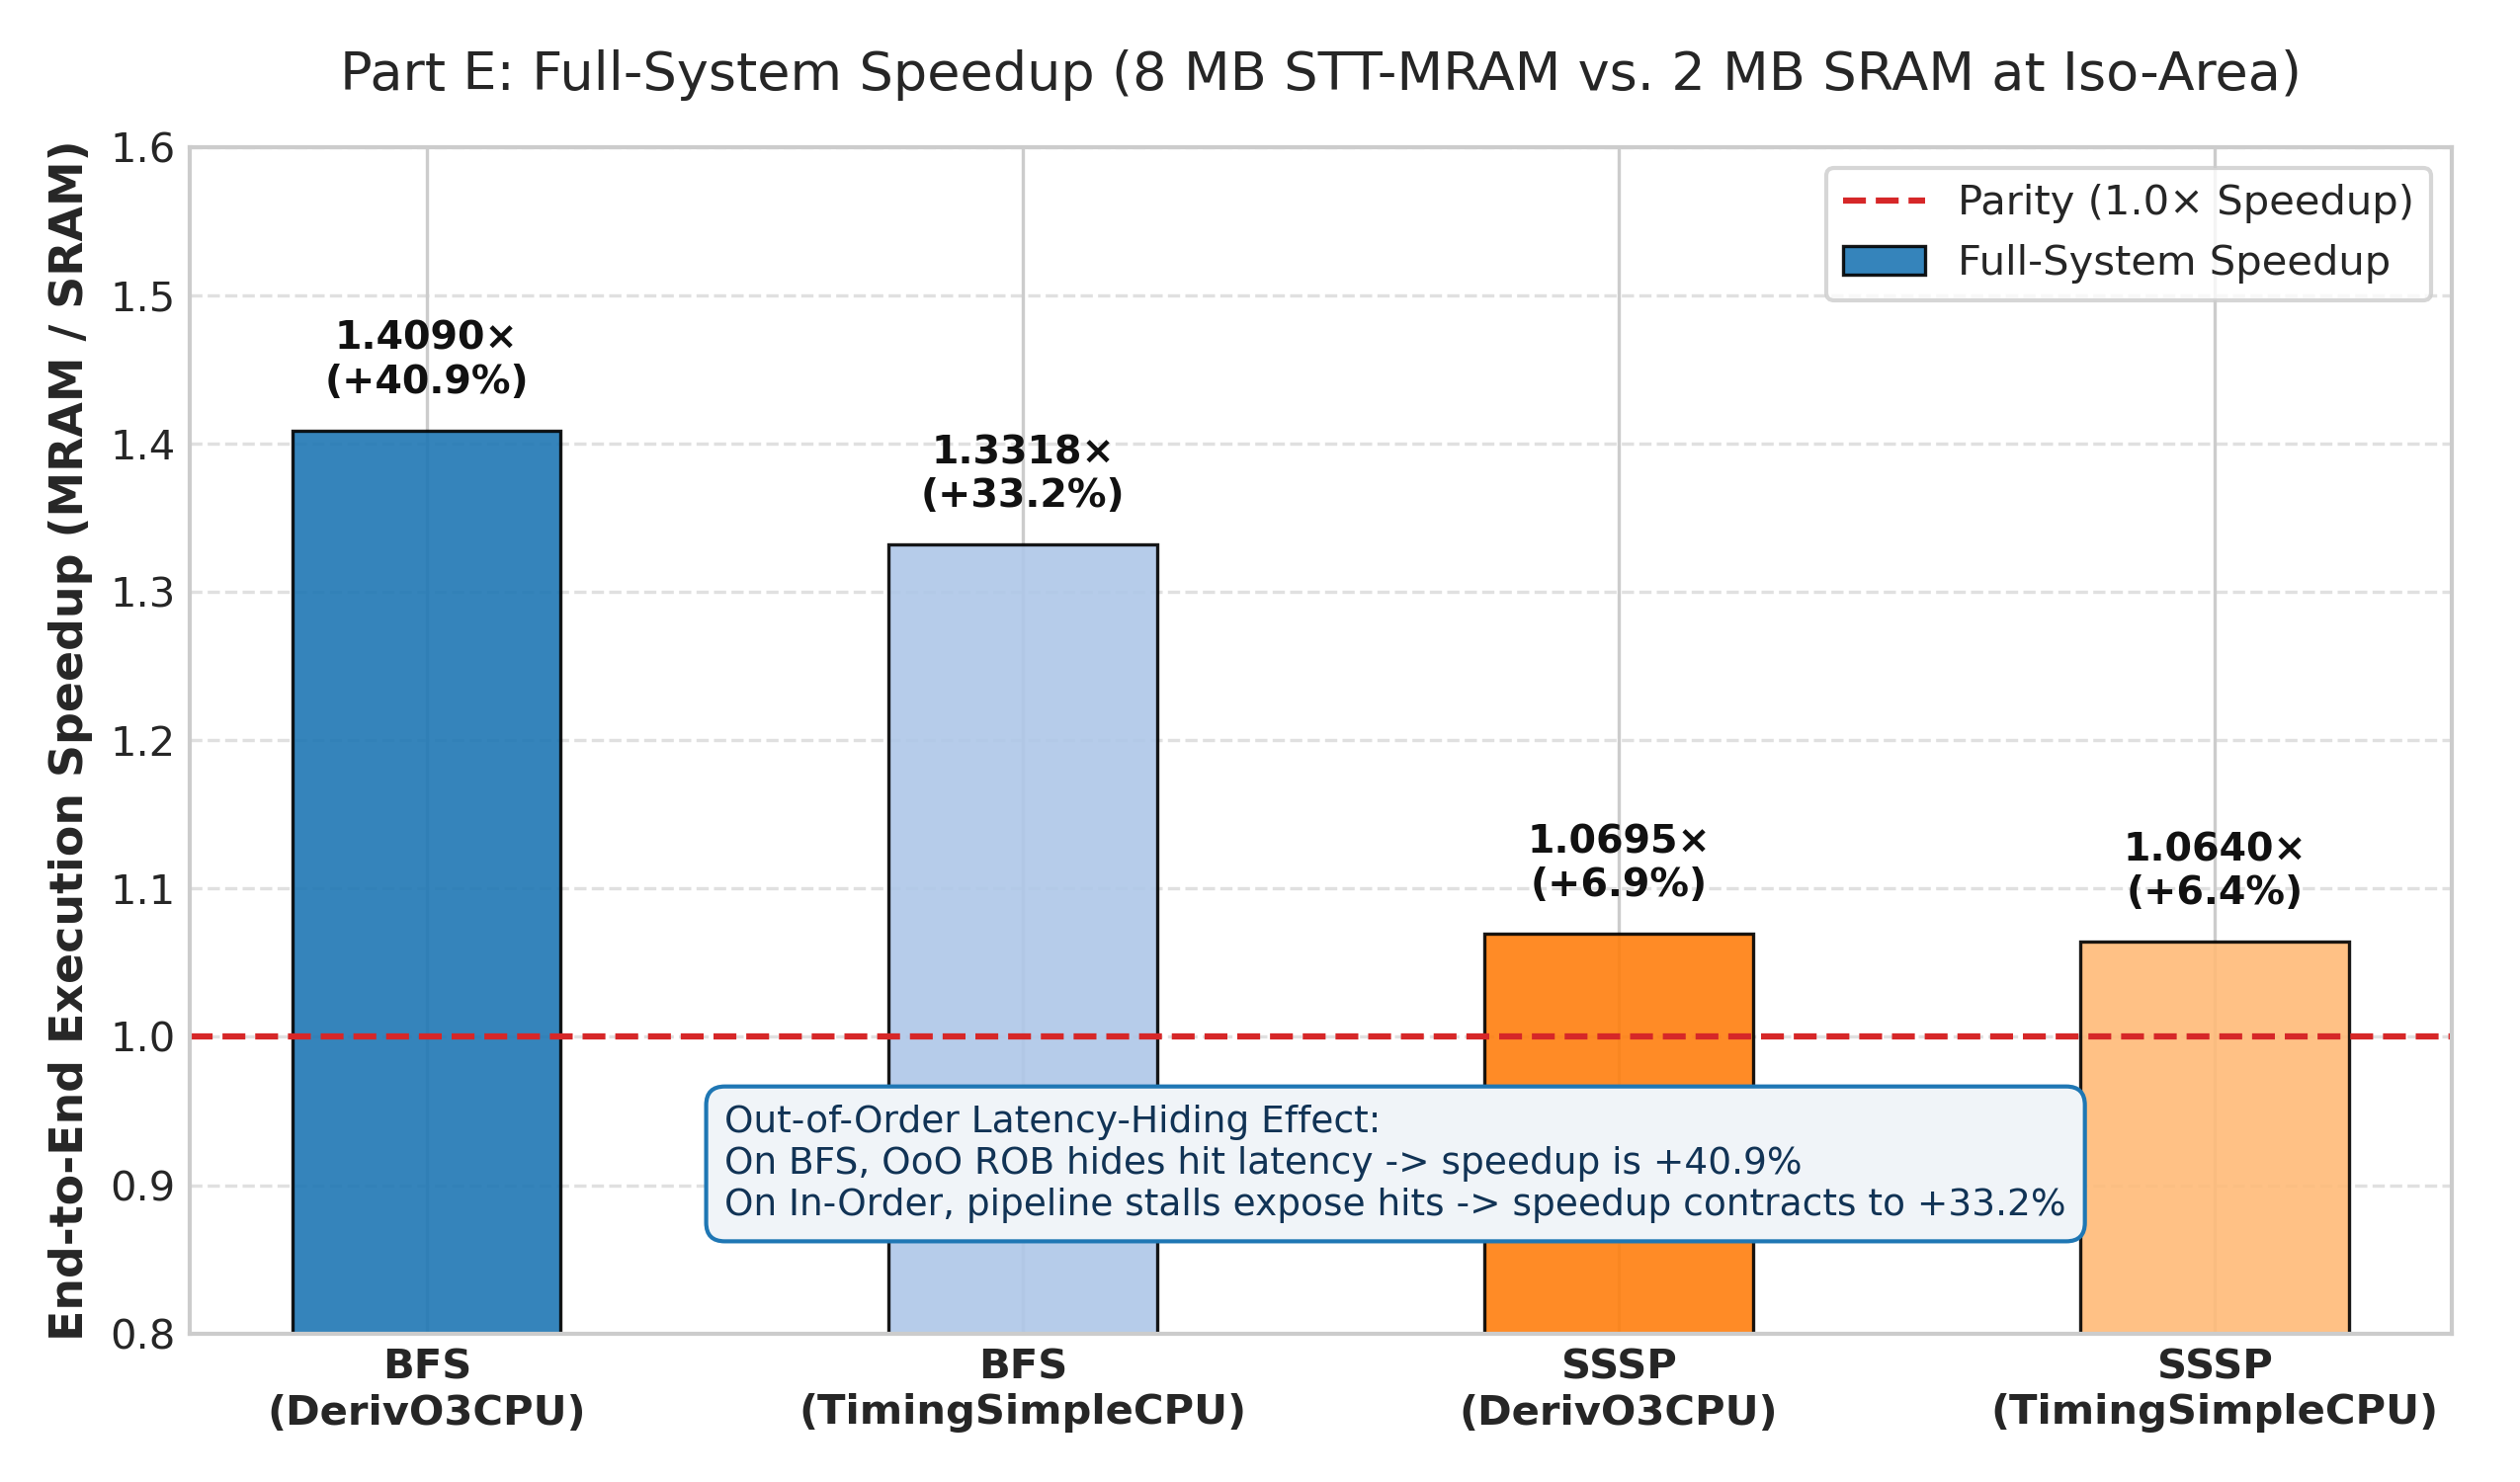
\includegraphics[width=0.6\textwidth]{plots/plot4_part_e_speedup_comparison.png}
    \caption{Speedup of 8\,MB STT-MRAM over 2\,MB SRAM on O3 vs In-Order cores.}
    \label{fig:plot4}
\end{figure}

\subsection*{Architectural Synthesis \& Deliverables (Task 4)}
\begin{itemize}
    \item \textbf{Central Question Answer:} "Should the 2 MB L2 cache in our accelerator be SRAM, or STT-MRAM?" \newline
Based on our cross-layer evaluation, the 8\,MB STT-MRAM is \textbf{1.409$\times$ faster} than the iso-area 2\,MB SRAM for the BFS workload when paired with an Out-of-Order core. While STT-MRAM suffers from a 3.91$\times$ worse write latency (NVSim) and a 14-cycle read latency (CACTI vs NVSim), the massive 4$\times$ density advantage allows the 8\,MB capacity to collapse the L2 miss rate from 68.7\% to 18.2\% (gem5). This prevents the DDR4 memory channel from choking on row conflicts (Ramulator), provided the core has enough out-of-order resources to mask the sluggish 14-cycle array responses.

\item \textbf{Reviewer Assumptions to Attack:} If I were a reviewer, the first assumption I would attack is the \textbf{write endurance and wear-leveling}. Graph analytics algorithms (like SSSP) generate intense, localized write traffic, and STT-MRAM has finite write endurance which gem5 and NVSim ignored. Second, I would attack the \textbf{fixed 14-cycle L2 hit latency assumption}; since writes take 10.3\,ns (Part C), a read arriving during a long write will be blocked, causing dynamic congestion that simple latency assignment misses. Third, I would challenge the \textbf{thermal reliability}. As shown in Part A, SRAM degrades at $85\,^{\circ}$C. STT-MRAM retention time is exponentially sensitive to temperature, meaning an 8\,MB high-performance L2 might suffer thermal failure or require constant refresh operations that the models omitted. One more thing I would challenge is this is focused for a single graph workload benchmark. We can't conclude that STT-MRAM is better than SRAM for all graph workloads.

\end{itemize}
\end{document}
